
\begin{tikzpicture}[scale=5]

    \begin{scope}[
            yshift=-3.5, xshift=16, every node/.append style={
            yslant=-0,xslant=0},yslant=0,xslant=0]
            
    \node[
          opacity=0.5, anchor=south east,inner sep=0pt] at (0,0) 
           {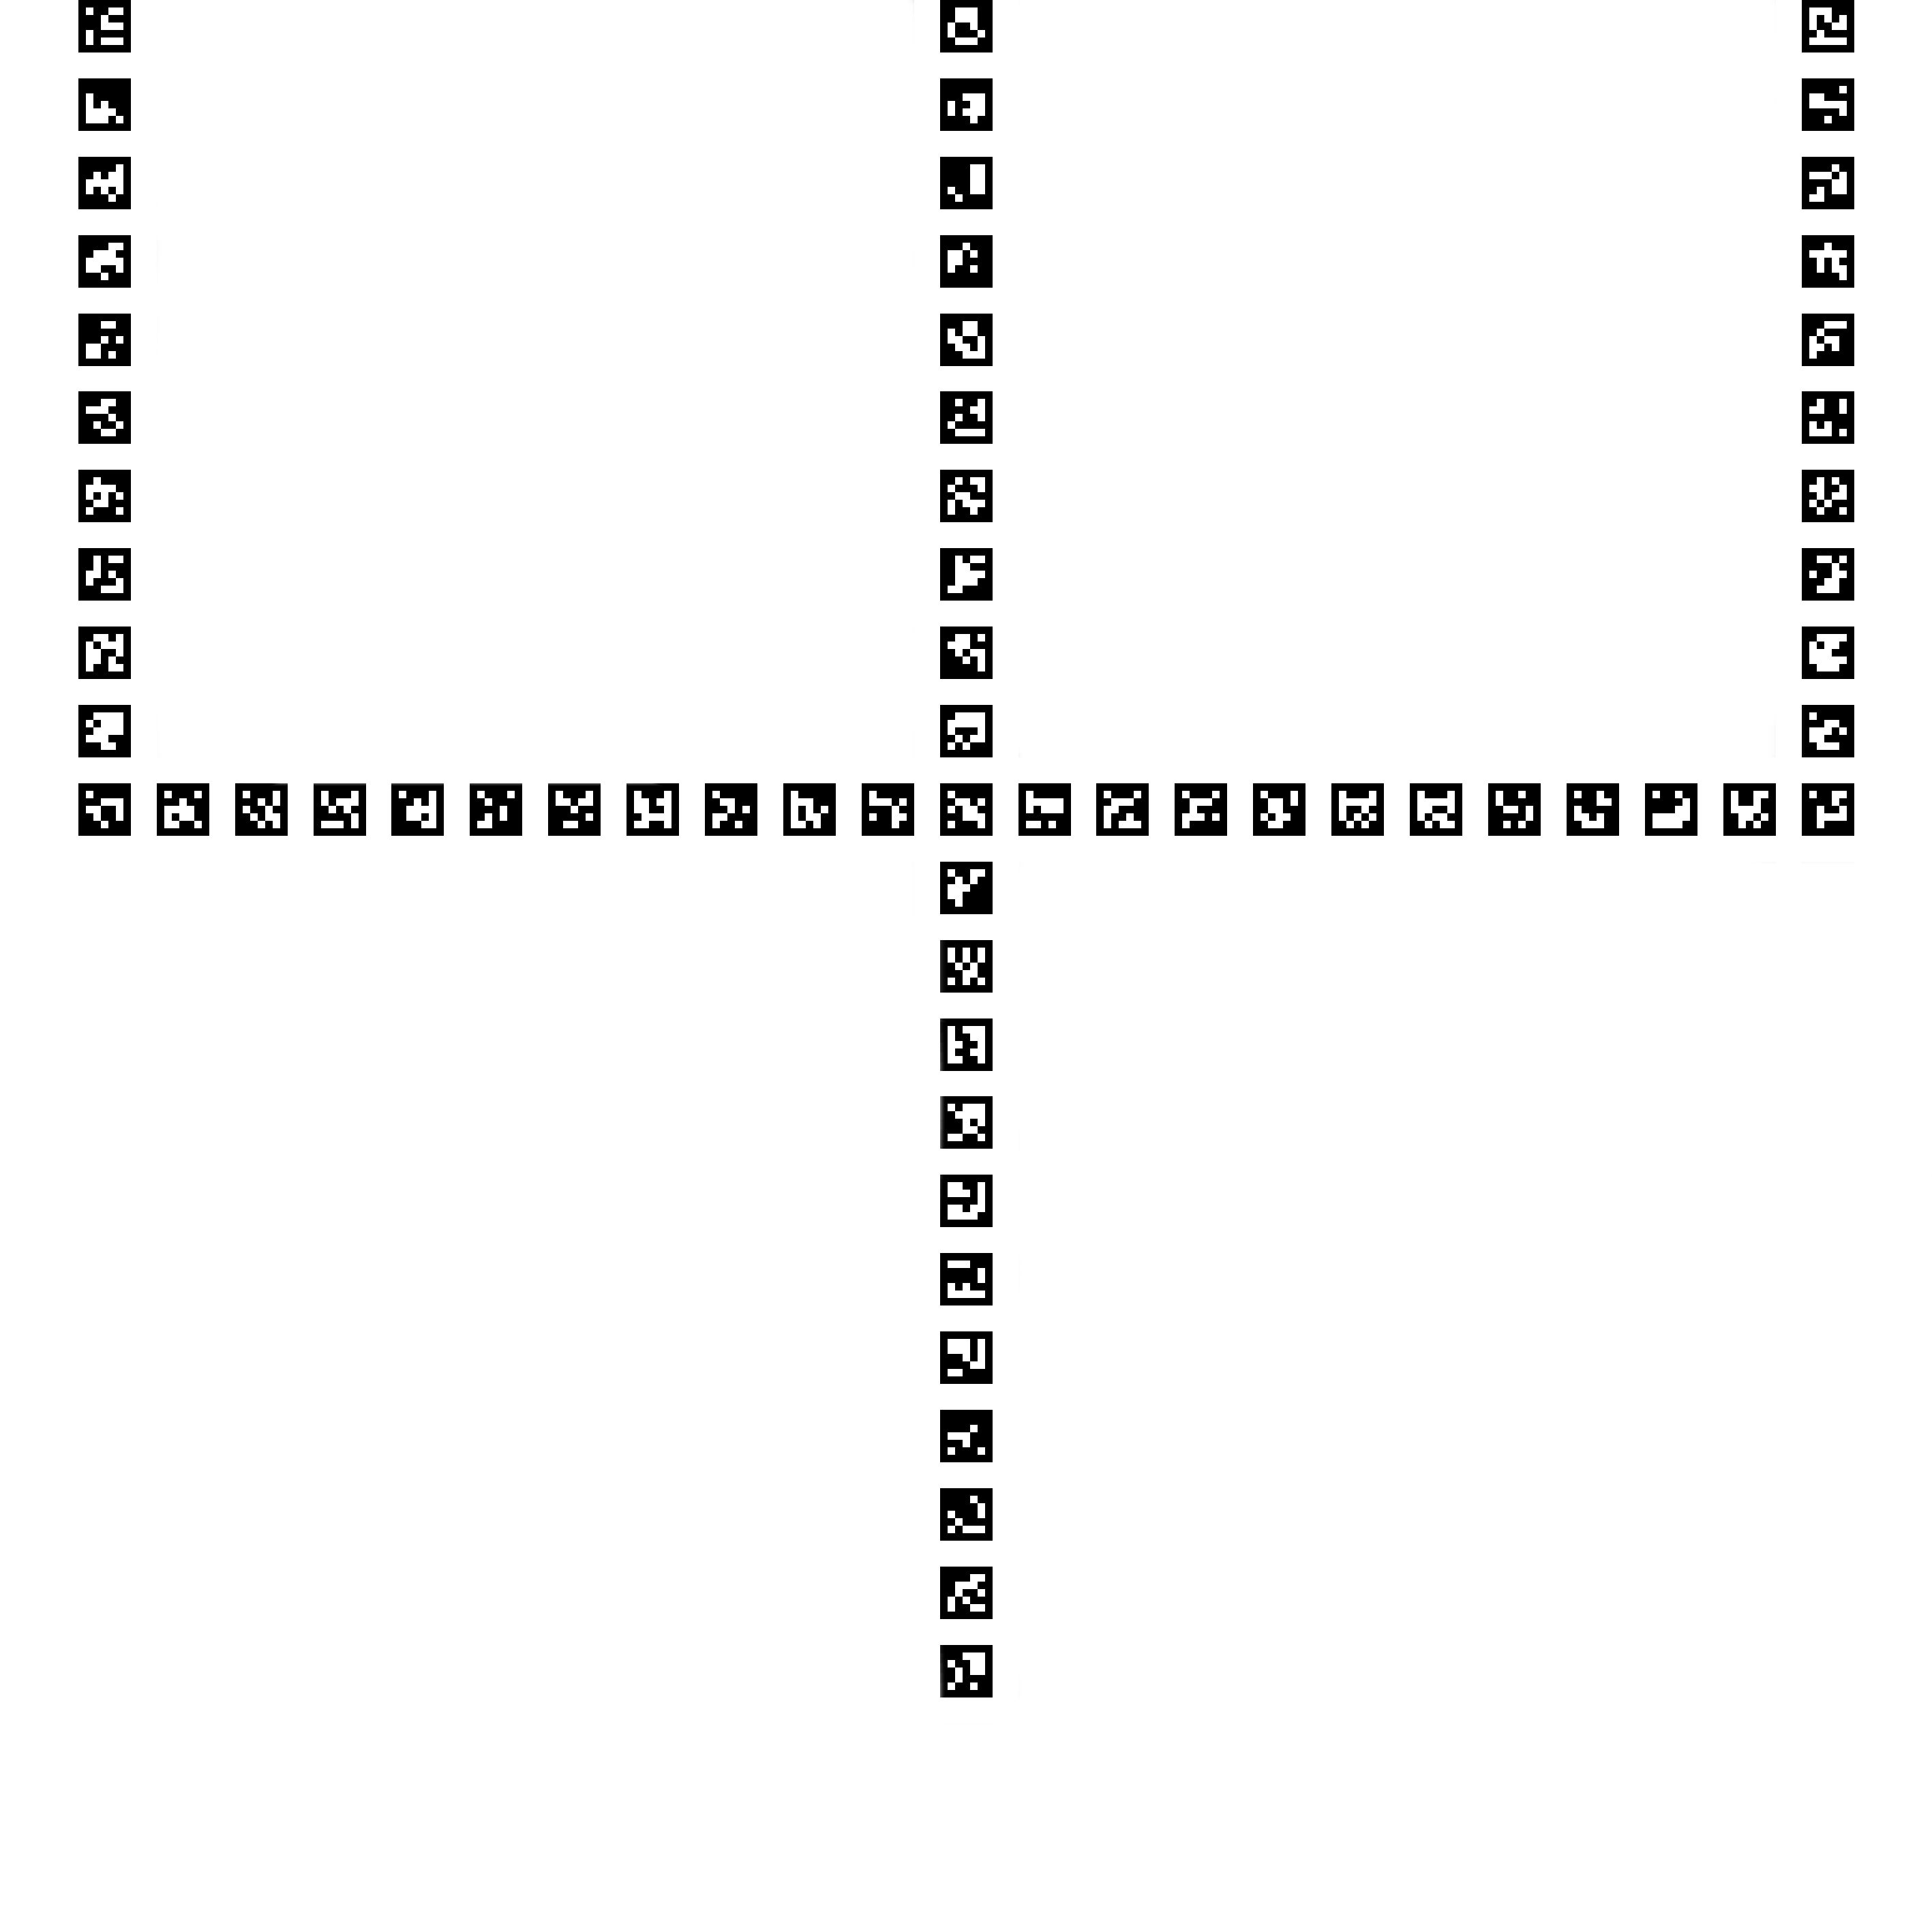
\includegraphics[width=6cm]{../Figures/original_one_pattern_aruco.png}}; 

    \end{scope}

%Draw ground marker (world)
\draw[->, red] (-0.6,0) -- (-0.3,0) node[right]{$x$};
\draw[->, green] (-0.6,0) -- (-0.6,0.3) node[above]{$y$};
\node[align=center] at (-1.0, 0.2) (ori) {$Marker_{ground}$};
\draw[->,help lines,shorten >=3pt] (ori) .. controls (-0.8,0.13) and (-0.75, 0.1) .. (-0.61, 0.02);

%Draw GPS to vision marker
\draw[->, red] (-0.1,0.35) -- (0.2,0.35) node[right]{$x$};
\draw[->, blue] (-0.1,0.35) -- (-0.1,0.05) node[below]{$z$};
\node[align=center] at (0.4, 0.1) (ori) {$Marker_{GPS2vision}$};
\draw[->, black, help lines,shorten >=3pt] (ori) .. controls (0.2,0.15) and (0.1, 0.2) .. (-0.1, 0.35);

%Draw landing marker one
\draw[->, red] (-0.62,1.30) -- (-0.32,1.3) node[right]{$x$};
\draw[->, blue] (-0.62,1.30) -- (-0.62,1.0) node[below]{$z$};
\node[align=center] at (-1.1, 1.0) (ori) {$Marker_{landing_1}$};
\draw[->, black, help lines,shorten >=3pt] (ori) .. controls (-1.0,1.1) and (-0.95, 1.2) .. (-0.62, 1.30);

%Draw Glanding marker two
\draw[->, red] (-0.08,1.3) -- (0.18,1.3) node[right]{$x$};
\draw[->, blue] (-0.08,1.3) -- (-0.08,1.0) node[below]{$z$};
\node[align=center] at (0.4, 1.5) (ori) {$Marker_{landing_2}$};
\draw[->, black, help lines,shorten >=3pt] (ori) .. controls (0.4,1.4) and (0.0, 1.4) .. (-0.076, 1.3);

%Draw Glanding marker two
\draw[->, red] (0.45,1.3) -- (0.75,1.3) node[right]{$x$};
\draw[->, blue] (0.45,1.3) -- (0.45,1.0) node[below]{$z$};
\node[align=center] at (1.0, 1.1) (ori) {$Marker_{landing_3}$};
\draw[->, black, help lines,shorten >=3pt] (ori) .. controls (0.6,1.1) and (0.7, 1.22) .. (0.45, 1.28);

\end{tikzpicture}